% Options for packages loaded elsewhere
\PassOptionsToPackage{unicode}{hyperref}
\PassOptionsToPackage{hyphens}{url}
\PassOptionsToPackage{dvipsnames,svgnames,x11names}{xcolor}
%
\documentclass[
  letterpaper,
  DIV=11,
  numbers=noendperiod]{scrreprt}

\usepackage{amsmath,amssymb}
\usepackage{lmodern}
\usepackage{iftex}
\ifPDFTeX
  \usepackage[T1]{fontenc}
  \usepackage[utf8]{inputenc}
  \usepackage{textcomp} % provide euro and other symbols
\else % if luatex or xetex
  \usepackage{unicode-math}
  \defaultfontfeatures{Scale=MatchLowercase}
  \defaultfontfeatures[\rmfamily]{Ligatures=TeX,Scale=1}
\fi
% Use upquote if available, for straight quotes in verbatim environments
\IfFileExists{upquote.sty}{\usepackage{upquote}}{}
\IfFileExists{microtype.sty}{% use microtype if available
  \usepackage[]{microtype}
  \UseMicrotypeSet[protrusion]{basicmath} % disable protrusion for tt fonts
}{}
\makeatletter
\@ifundefined{KOMAClassName}{% if non-KOMA class
  \IfFileExists{parskip.sty}{%
    \usepackage{parskip}
  }{% else
    \setlength{\parindent}{0pt}
    \setlength{\parskip}{6pt plus 2pt minus 1pt}}
}{% if KOMA class
  \KOMAoptions{parskip=half}}
\makeatother
\usepackage{xcolor}
\setlength{\emergencystretch}{3em} % prevent overfull lines
\setcounter{secnumdepth}{5}
% Make \paragraph and \subparagraph free-standing
\ifx\paragraph\undefined\else
  \let\oldparagraph\paragraph
  \renewcommand{\paragraph}[1]{\oldparagraph{#1}\mbox{}}
\fi
\ifx\subparagraph\undefined\else
  \let\oldsubparagraph\subparagraph
  \renewcommand{\subparagraph}[1]{\oldsubparagraph{#1}\mbox{}}
\fi

\usepackage{color}
\usepackage{fancyvrb}
\newcommand{\VerbBar}{|}
\newcommand{\VERB}{\Verb[commandchars=\\\{\}]}
\DefineVerbatimEnvironment{Highlighting}{Verbatim}{commandchars=\\\{\}}
% Add ',fontsize=\small' for more characters per line
\usepackage{framed}
\definecolor{shadecolor}{RGB}{241,243,245}
\newenvironment{Shaded}{\begin{snugshade}}{\end{snugshade}}
\newcommand{\AlertTok}[1]{\textcolor[rgb]{0.68,0.00,0.00}{#1}}
\newcommand{\AnnotationTok}[1]{\textcolor[rgb]{0.37,0.37,0.37}{#1}}
\newcommand{\AttributeTok}[1]{\textcolor[rgb]{0.40,0.45,0.13}{#1}}
\newcommand{\BaseNTok}[1]{\textcolor[rgb]{0.68,0.00,0.00}{#1}}
\newcommand{\BuiltInTok}[1]{\textcolor[rgb]{0.00,0.23,0.31}{#1}}
\newcommand{\CharTok}[1]{\textcolor[rgb]{0.13,0.47,0.30}{#1}}
\newcommand{\CommentTok}[1]{\textcolor[rgb]{0.37,0.37,0.37}{#1}}
\newcommand{\CommentVarTok}[1]{\textcolor[rgb]{0.37,0.37,0.37}{\textit{#1}}}
\newcommand{\ConstantTok}[1]{\textcolor[rgb]{0.56,0.35,0.01}{#1}}
\newcommand{\ControlFlowTok}[1]{\textcolor[rgb]{0.00,0.23,0.31}{#1}}
\newcommand{\DataTypeTok}[1]{\textcolor[rgb]{0.68,0.00,0.00}{#1}}
\newcommand{\DecValTok}[1]{\textcolor[rgb]{0.68,0.00,0.00}{#1}}
\newcommand{\DocumentationTok}[1]{\textcolor[rgb]{0.37,0.37,0.37}{\textit{#1}}}
\newcommand{\ErrorTok}[1]{\textcolor[rgb]{0.68,0.00,0.00}{#1}}
\newcommand{\ExtensionTok}[1]{\textcolor[rgb]{0.00,0.23,0.31}{#1}}
\newcommand{\FloatTok}[1]{\textcolor[rgb]{0.68,0.00,0.00}{#1}}
\newcommand{\FunctionTok}[1]{\textcolor[rgb]{0.28,0.35,0.67}{#1}}
\newcommand{\ImportTok}[1]{\textcolor[rgb]{0.00,0.46,0.62}{#1}}
\newcommand{\InformationTok}[1]{\textcolor[rgb]{0.37,0.37,0.37}{#1}}
\newcommand{\KeywordTok}[1]{\textcolor[rgb]{0.00,0.23,0.31}{#1}}
\newcommand{\NormalTok}[1]{\textcolor[rgb]{0.00,0.23,0.31}{#1}}
\newcommand{\OperatorTok}[1]{\textcolor[rgb]{0.37,0.37,0.37}{#1}}
\newcommand{\OtherTok}[1]{\textcolor[rgb]{0.00,0.23,0.31}{#1}}
\newcommand{\PreprocessorTok}[1]{\textcolor[rgb]{0.68,0.00,0.00}{#1}}
\newcommand{\RegionMarkerTok}[1]{\textcolor[rgb]{0.00,0.23,0.31}{#1}}
\newcommand{\SpecialCharTok}[1]{\textcolor[rgb]{0.37,0.37,0.37}{#1}}
\newcommand{\SpecialStringTok}[1]{\textcolor[rgb]{0.13,0.47,0.30}{#1}}
\newcommand{\StringTok}[1]{\textcolor[rgb]{0.13,0.47,0.30}{#1}}
\newcommand{\VariableTok}[1]{\textcolor[rgb]{0.07,0.07,0.07}{#1}}
\newcommand{\VerbatimStringTok}[1]{\textcolor[rgb]{0.13,0.47,0.30}{#1}}
\newcommand{\WarningTok}[1]{\textcolor[rgb]{0.37,0.37,0.37}{\textit{#1}}}

\providecommand{\tightlist}{%
  \setlength{\itemsep}{0pt}\setlength{\parskip}{0pt}}\usepackage{longtable,booktabs,array}
\usepackage{calc} % for calculating minipage widths
% Correct order of tables after \paragraph or \subparagraph
\usepackage{etoolbox}
\makeatletter
\patchcmd\longtable{\par}{\if@noskipsec\mbox{}\fi\par}{}{}
\makeatother
% Allow footnotes in longtable head/foot
\IfFileExists{footnotehyper.sty}{\usepackage{footnotehyper}}{\usepackage{footnote}}
\makesavenoteenv{longtable}
\usepackage{graphicx}
\makeatletter
\def\maxwidth{\ifdim\Gin@nat@width>\linewidth\linewidth\else\Gin@nat@width\fi}
\def\maxheight{\ifdim\Gin@nat@height>\textheight\textheight\else\Gin@nat@height\fi}
\makeatother
% Scale images if necessary, so that they will not overflow the page
% margins by default, and it is still possible to overwrite the defaults
% using explicit options in \includegraphics[width, height, ...]{}
\setkeys{Gin}{width=\maxwidth,height=\maxheight,keepaspectratio}
% Set default figure placement to htbp
\makeatletter
\def\fps@figure{htbp}
\makeatother
\newlength{\cslhangindent}
\setlength{\cslhangindent}{1.5em}
\newlength{\csllabelwidth}
\setlength{\csllabelwidth}{3em}
\newlength{\cslentryspacingunit} % times entry-spacing
\setlength{\cslentryspacingunit}{\parskip}
\newenvironment{CSLReferences}[2] % #1 hanging-ident, #2 entry spacing
 {% don't indent paragraphs
  \setlength{\parindent}{0pt}
  % turn on hanging indent if param 1 is 1
  \ifodd #1
  \let\oldpar\par
  \def\par{\hangindent=\cslhangindent\oldpar}
  \fi
  % set entry spacing
  \setlength{\parskip}{#2\cslentryspacingunit}
 }%
 {}
\usepackage{calc}
\newcommand{\CSLBlock}[1]{#1\hfill\break}
\newcommand{\CSLLeftMargin}[1]{\parbox[t]{\csllabelwidth}{#1}}
\newcommand{\CSLRightInline}[1]{\parbox[t]{\linewidth - \csllabelwidth}{#1}\break}
\newcommand{\CSLIndent}[1]{\hspace{\cslhangindent}#1}

\usepackage{booktabs}
\usepackage{longtable}
\usepackage{array}
\usepackage{multirow}
\usepackage{wrapfig}
\usepackage{float}
\usepackage{colortbl}
\usepackage{pdflscape}
\usepackage{tabu}
\usepackage{threeparttable}
\usepackage{threeparttablex}
\usepackage[normalem]{ulem}
\usepackage{makecell}
\usepackage{xcolor}
\KOMAoption{captions}{tableheading}
\makeatletter
\makeatother
\makeatletter
\@ifpackageloaded{bookmark}{}{\usepackage{bookmark}}
\makeatother
\makeatletter
\@ifpackageloaded{caption}{}{\usepackage{caption}}
\AtBeginDocument{%
\ifdefined\contentsname
  \renewcommand*\contentsname{Table of contents}
\else
  \newcommand\contentsname{Table of contents}
\fi
\ifdefined\listfigurename
  \renewcommand*\listfigurename{List of Figures}
\else
  \newcommand\listfigurename{List of Figures}
\fi
\ifdefined\listtablename
  \renewcommand*\listtablename{List of Tables}
\else
  \newcommand\listtablename{List of Tables}
\fi
\ifdefined\figurename
  \renewcommand*\figurename{Figure}
\else
  \newcommand\figurename{Figure}
\fi
\ifdefined\tablename
  \renewcommand*\tablename{Table}
\else
  \newcommand\tablename{Table}
\fi
}
\@ifpackageloaded{float}{}{\usepackage{float}}
\floatstyle{ruled}
\@ifundefined{c@chapter}{\newfloat{codelisting}{h}{lop}}{\newfloat{codelisting}{h}{lop}[chapter]}
\floatname{codelisting}{Listing}
\newcommand*\listoflistings{\listof{codelisting}{List of Listings}}
\makeatother
\makeatletter
\@ifpackageloaded{caption}{}{\usepackage{caption}}
\@ifpackageloaded{subcaption}{}{\usepackage{subcaption}}
\makeatother
\makeatletter
\@ifpackageloaded{tcolorbox}{}{\usepackage[many]{tcolorbox}}
\makeatother
\makeatletter
\@ifundefined{shadecolor}{\definecolor{shadecolor}{rgb}{.97, .97, .97}}
\makeatother
\makeatletter
\makeatother
\ifLuaTeX
  \usepackage{selnolig}  % disable illegal ligatures
\fi
\IfFileExists{bookmark.sty}{\usepackage{bookmark}}{\usepackage{hyperref}}
\IfFileExists{xurl.sty}{\usepackage{xurl}}{} % add URL line breaks if available
\urlstyle{same} % disable monospaced font for URLs
\hypersetup{
  pdftitle={Spatial Modelling for Data Scientists},
  pdfauthor={Francisco Rowe, Dani Arribas-Bel},
  colorlinks=true,
  linkcolor={blue},
  filecolor={Maroon},
  citecolor={Blue},
  urlcolor={Blue},
  pdfcreator={LaTeX via pandoc}}

\title{Spatial Modelling for Data Scientists}
\author{Francisco Rowe, Dani Arribas-Bel}
\date{November 6, 2022}

\begin{document}
\maketitle
\ifdefined\Shaded\renewenvironment{Shaded}{\begin{tcolorbox}[sharp corners, interior hidden, borderline west={3pt}{0pt}{shadecolor}, enhanced, frame hidden, breakable, boxrule=0pt]}{\end{tcolorbox}}\fi

\renewcommand*\contentsname{Table of contents}
{
\hypersetup{linkcolor=}
\setcounter{tocdepth}{2}
\tableofcontents
}
\bookmarksetup{startatroot}

\hypertarget{welcome}{%
\chapter*{Welcome}\label{welcome}}
\addcontentsline{toc}{chapter}{Welcome}

This is the new website for \textbf{``Spatial Modeling for Data
Scientists''} taught by Dr.~Francisco Rowe at the University of
Liverpool, United Kingdom. The website is \emph{work in progress} and
will be fully updated by February 1st 2023. The course provides an
intuitive understanding of models and analytical approaches to
manipulate, visualise and interrogate spatial data.

The website is licensed under the
\href{https://creativecommons.org/licenses/by-nc-nd/4.0/}{Attribution-NonCommercial-NoDerivatives
4.0 International} License. A compilation of this web course is hosted
as a GitHub repository that you can access:

\begin{itemize}
\tightlist
\item
  As a
  \href{https://github.com/fcorowe/smds/archive/refs/heads/main.zip}{download}
  of a \texttt{.zip} file that contains all the materials.
\item
  As an \href{}{html website}.
\item
  As a \href{}{pdf document}
\item
  As a \href{https://github.com/fcorowe/smds}{GitHub repository}.
\end{itemize}

\hypertarget{contact}{%
\section*{Contact}\label{contact}}
\addcontentsline{toc}{section}{Contact}

\begin{quote}
Francisco Rowe - \texttt{F.Rowe-Gonzalez\ {[}at{]}\ liverpool.ac.uk}\\
Senior Lecturer in Quantitative Human Geography\\
Office 507, Roxby Building,\\
University of Liverpool - 74 Bedford St S,\\
Liverpool, L69 7ZT,\\
United Kingdom.
\end{quote}

\bookmarksetup{startatroot}

\hypertarget{overview}{%
\chapter{Overview}\label{overview}}

Access to all materials, including lecture notes, computational
notebooks and datasets, is centralised through the use of the course
website available in the following url:

\begin{quote}
\url{https://gdsl-ul.github.io/san/}
\end{quote}

The module handbook, including the assessment description, criteria and
module programme, and videos for each teaching week can be accessed via
the module Canvas site:

\begin{quote}
\href{https://liverpool.instructure.com}{ENS453 Spatial Modelling for
Data Scientists}
\end{quote}

\hypertarget{aims}{%
\section{Aims}\label{aims}}

This module aims to provides students with a range of techniques for
analysing and modelling spatial data:

\begin{itemize}
\tightlist
\item
  build upon the more general research training delivered via companion
  modules on \emph{Data Collection and Data Analysis}, both of which
  have an aspatial focus;
\item
  highlight a number of key social issues that have a spatial dimension;
\item
  explain the specific challenges faced when attempting to analyse
  spatial data;
\item
  introduce a range of analytical techniques and approaches suitable for
  the analysis of spatial data; and,
\item
  enhance practical skills in using \emph{R} software packages to
  implement a wide range of spatial analytical tools.
\end{itemize}

\hypertarget{learning-outcomes}{%
\section{Learning Outcomes}\label{learning-outcomes}}

By the end of the module, students should be able to:

\begin{itemize}
\tightlist
\item
  identify some key sources of spatial data and resources of spatial
  analysis and modelling tools;
\item
  explain the advantages of taking spatial structure into account when
  analysing spatial data;
\item
  apply a range of computer-based techniques for the analysis of spatial
  data, including mapping, correlation, kernel density estimation,
  regression, multi-level models, geographically-weighted regression,
  spatial interaction models and spatial econometrics;
\item
  apply appropriate analytical strategies to tackle the key
  methodological challenges facing spatial analysis -- spatial
  autocorrelation, heterogeneity, and ecological fallacy; and,
\item
  select appropriate analytical tools for analysing specific spatial
  data sets to address emerging social issues facing the society.
\end{itemize}

\hypertarget{feedback}{%
\section{Feedback}\label{feedback}}

\begin{itemize}
\item
  \emph{Formal assessment of two computational essays}. Written
  assignment-specific feedback will be provided within three working
  weeks of the submission deadline. Comments will offer an understanding
  of the mark awarded and identify areas which can be considered for
  improvement in future assignments.
\item
  \emph{Verbal face-to-face feedback}. Immediate face-to-face feedback
  will be provided during lecture, discussion and clinic sessions in
  interaction with staff. This will take place in all live sessions
  during the semester.
\item
  \emph{Online forum}. Asynchronous written feedback will be provided
  via an online forum maintained by the module lead. Students are
  encouraged to contribute by asking and answering questions relating to
  the module content. Staff will monitor the forum Monday to Friday
  9am-5pm, but it will be open to students to make contributions at all
  times.
\end{itemize}

\hypertarget{computational-environment}{%
\section{Computational Environment}\label{computational-environment}}

To reproduce the code in the book, you need the most recent version of R
and packages. These can be installed following the instructions provided
in our \href{https://gdsl-ul.github.io/r_install/}{R installation
guide}.

\hypertarget{dependency-list}{%
\subsection{Dependency list}\label{dependency-list}}

The list of libraries used in this book is provided below. If you have
followed the instructions provided in our
\href{https://gdsl-ul.github.io/r_install/}{R installation guide} and
will be using Docker, you can relax and these libraries have already
been installed for you.

If you have \texttt{natively} installed R and RStudio, you need to
ensure you have installed the list of libraries used in this book
following the steps provided
\href{https://gdsl-ul.github.io/r_install/otherWin.html\#install-packages}{here}.

\begin{itemize}
\tightlist
\item
  \texttt{arm}
\item
  \texttt{car}
\item
  \texttt{corrplot}
\item
  \texttt{FRK}
\item
  \texttt{gghighlight}
\item
  \texttt{ggplot2}
\item
  \texttt{ggmap}
\item
  \texttt{GISTools}
\item
  \texttt{gridExtra}
\item
  \texttt{gstat}
\item
  \texttt{jtools}
\item
  \texttt{kableExtra}
\item
  \texttt{knitr}
\item
  \texttt{lme4}
\item
  \texttt{lmtest}
\item
  \texttt{lubridate}
\item
  \texttt{MASS}
\item
  \texttt{merTools}
\item
  \texttt{plyr}
\item
  \texttt{RColorBrewer}
\item
  \texttt{rgdal}
\item
  \texttt{sf}
\item
  \texttt{sjPlot}
\item
  \texttt{sp}
\item
  \texttt{spgwr}
\item
  \texttt{spatialreg}
\item
  \texttt{spacetime}
\item
  \texttt{stargazer}
\item
  \texttt{tidyverse}
\item
  \texttt{tmap}
\item
  \texttt{viridis}
\end{itemize}

\hypertarget{assessment}{%
\section{Assessment}\label{assessment}}

The final module mark is composed of the \emph{two computational
essays}. Together they are designed to cover the materials introduced in
the entirety of content covered during the semester. A computational
essay is an essay whose narrative is supported by code and computational
results that are included in the essay itself. Each teaching week, you
will be required to address a set of questions relating to the module
content covered in that week, and to use the material that you will
produce for this purpose to build your computational essay.

\textbf{Assignment 1 (50\%)} refer to the set of questions at the end of
Chapters @ref(points), @ref(flows) and @ref(spatialecon). You are
required to use your responses to build your computational essay. Each
chapter provides more specific guidance of the tasks and discussion that
you are required to consider in your assignment.

\textbf{Assignment 2 (50\%)} refer to the set of questions at the end of
Chapters @ref(mlm1), @ref(mlm2), @ref(gwr) and @ref(sta). You are
required to use your responses to build your computational essay. Each
chapter provides more specific guidance of the tasks and discussion that
you are required to consider in your assignment.

\hypertarget{format-requirements}{%
\subsection{Format Requirements}\label{format-requirements}}

Both assignments will have the same requirements:

\begin{itemize}
\tightlist
\item
  Maximum word count: 2,000 words, excluding figures and references.
\item
  Up to three maps, plot or figures (a figure may include more than one
  map and/or plot and will only count as one but needs to be integrated
  in the figure)
\item
  Up to two tables.
\end{itemize}

Assignments need to be prepared in \emph{R Notebook} format and then
converted into a self-contained \emph{HTML} file that will then be
submitted via Turnitin. The notebook should only display content that
will be assessed. Intermediate steps do not need to be displayed.
Messages resulting from loading packages, attaching data frames, or
similar messages do not need to be included as output code. Useful
resources to customise your \emph{R notebook} can be found on the
\href{https://rmarkdown.rstudio.com}{R Markdown website} from RStudio:\\
* \href{https://rmarkdown.rstudio.com/lesson-1.html}{A Guide}\\
* \href{https://bookdown.org/yihui/rmarkdown/}{R Markdown: The
Definitive Guide} by Xie, Allaire, and Grolemund (2018)\\
*
\href{https://rstudio.com/wp-content/uploads/2015/03/rmarkdown-reference.pdf?_ga=2.199646894.1496049738.1611760832-141828105.1610798362}{R
Markdown Reference Guide}

Two R Notebook templates will be available via the
\href{https://liverpool.instructure.com}{\emph{module Canvas site}}.

\emph{Submission} is electronic only via Turnitin on \emph{Canvas}.

\hypertarget{marking-criteria}{%
\subsection{Marking criteria}\label{marking-criteria}}

The Standard Environmental Sciences School marking criteria apply, with
a stronger emphasis on evidencing the use of regression models, critical
analysis of results and presentation standards. In addition to these
general criteria, the code and outputs (i.e.~tables, maps and plots)
contained within the notebook submitted for assessment will be assessed
according to the extent of documentation and evidence of expertise in
changing and extending the code options illustrated in each chapter.
Specifically, the following criteria will be applied:

\begin{itemize}
\tightlist
\item
  \textbf{0-15}: no documentation and use of default options.
\item
  \textbf{16-39}: little documentation and use of default options.
\item
  \textbf{40-49}: some documentation, and use of default options.
\item
  \textbf{50-59}: extensive documentation, and edit of some of the
  options provided in the notebook (e.g.~change north arrow location).
\item
  \textbf{60-69}: extensive well organised and easy to read
  documentation, and evidence of understanding of options provided in
  the code (e.g.~tweaking existing options).
\item
  \textbf{70-79}: all above, plus clear evidence of code design skills
  (e.g.~customising graphics, combining plots (or tables) into a single
  output, adding clear axis labels and variable names on graphic
  outputs, etc.).
\item
  \textbf{80-100}: all as above, plus code containing novel
  contributions that extend/improve the functionality the code was
  provided with (e.g.~comparative model assessments, novel methods to
  perform the task, etc.).
\end{itemize}

\bookmarksetup{startatroot}

\hypertarget{spatial_data}{%
\chapter{Spatial Data}\label{spatial_data}}

This Chapter seeks to present and describe distinctive attributes of
spatial data, and discuss some of the main challenges in analysing and
modelling these data. Spatial data is a term used to describe any data
associating a given variable attribute to a specific location on the
Earth's surface.

\hypertarget{spatial-data-types}{%
\section{Spatial Data types}\label{spatial-data-types}}

Different classifications of spatial data types exist. Knowing the
structure of the data at hand is important as specific analytical
methods would be more appropriate for particular data types. We will use
a particular classification involving four data types: lattice/areal
data, point data, flow data and trajectory data (Fig. 1). This is not a
exhaustive list but it is helpful to motivate the analytical and
modelling methods that we cover in this book.

\begin{figure}

{\centering 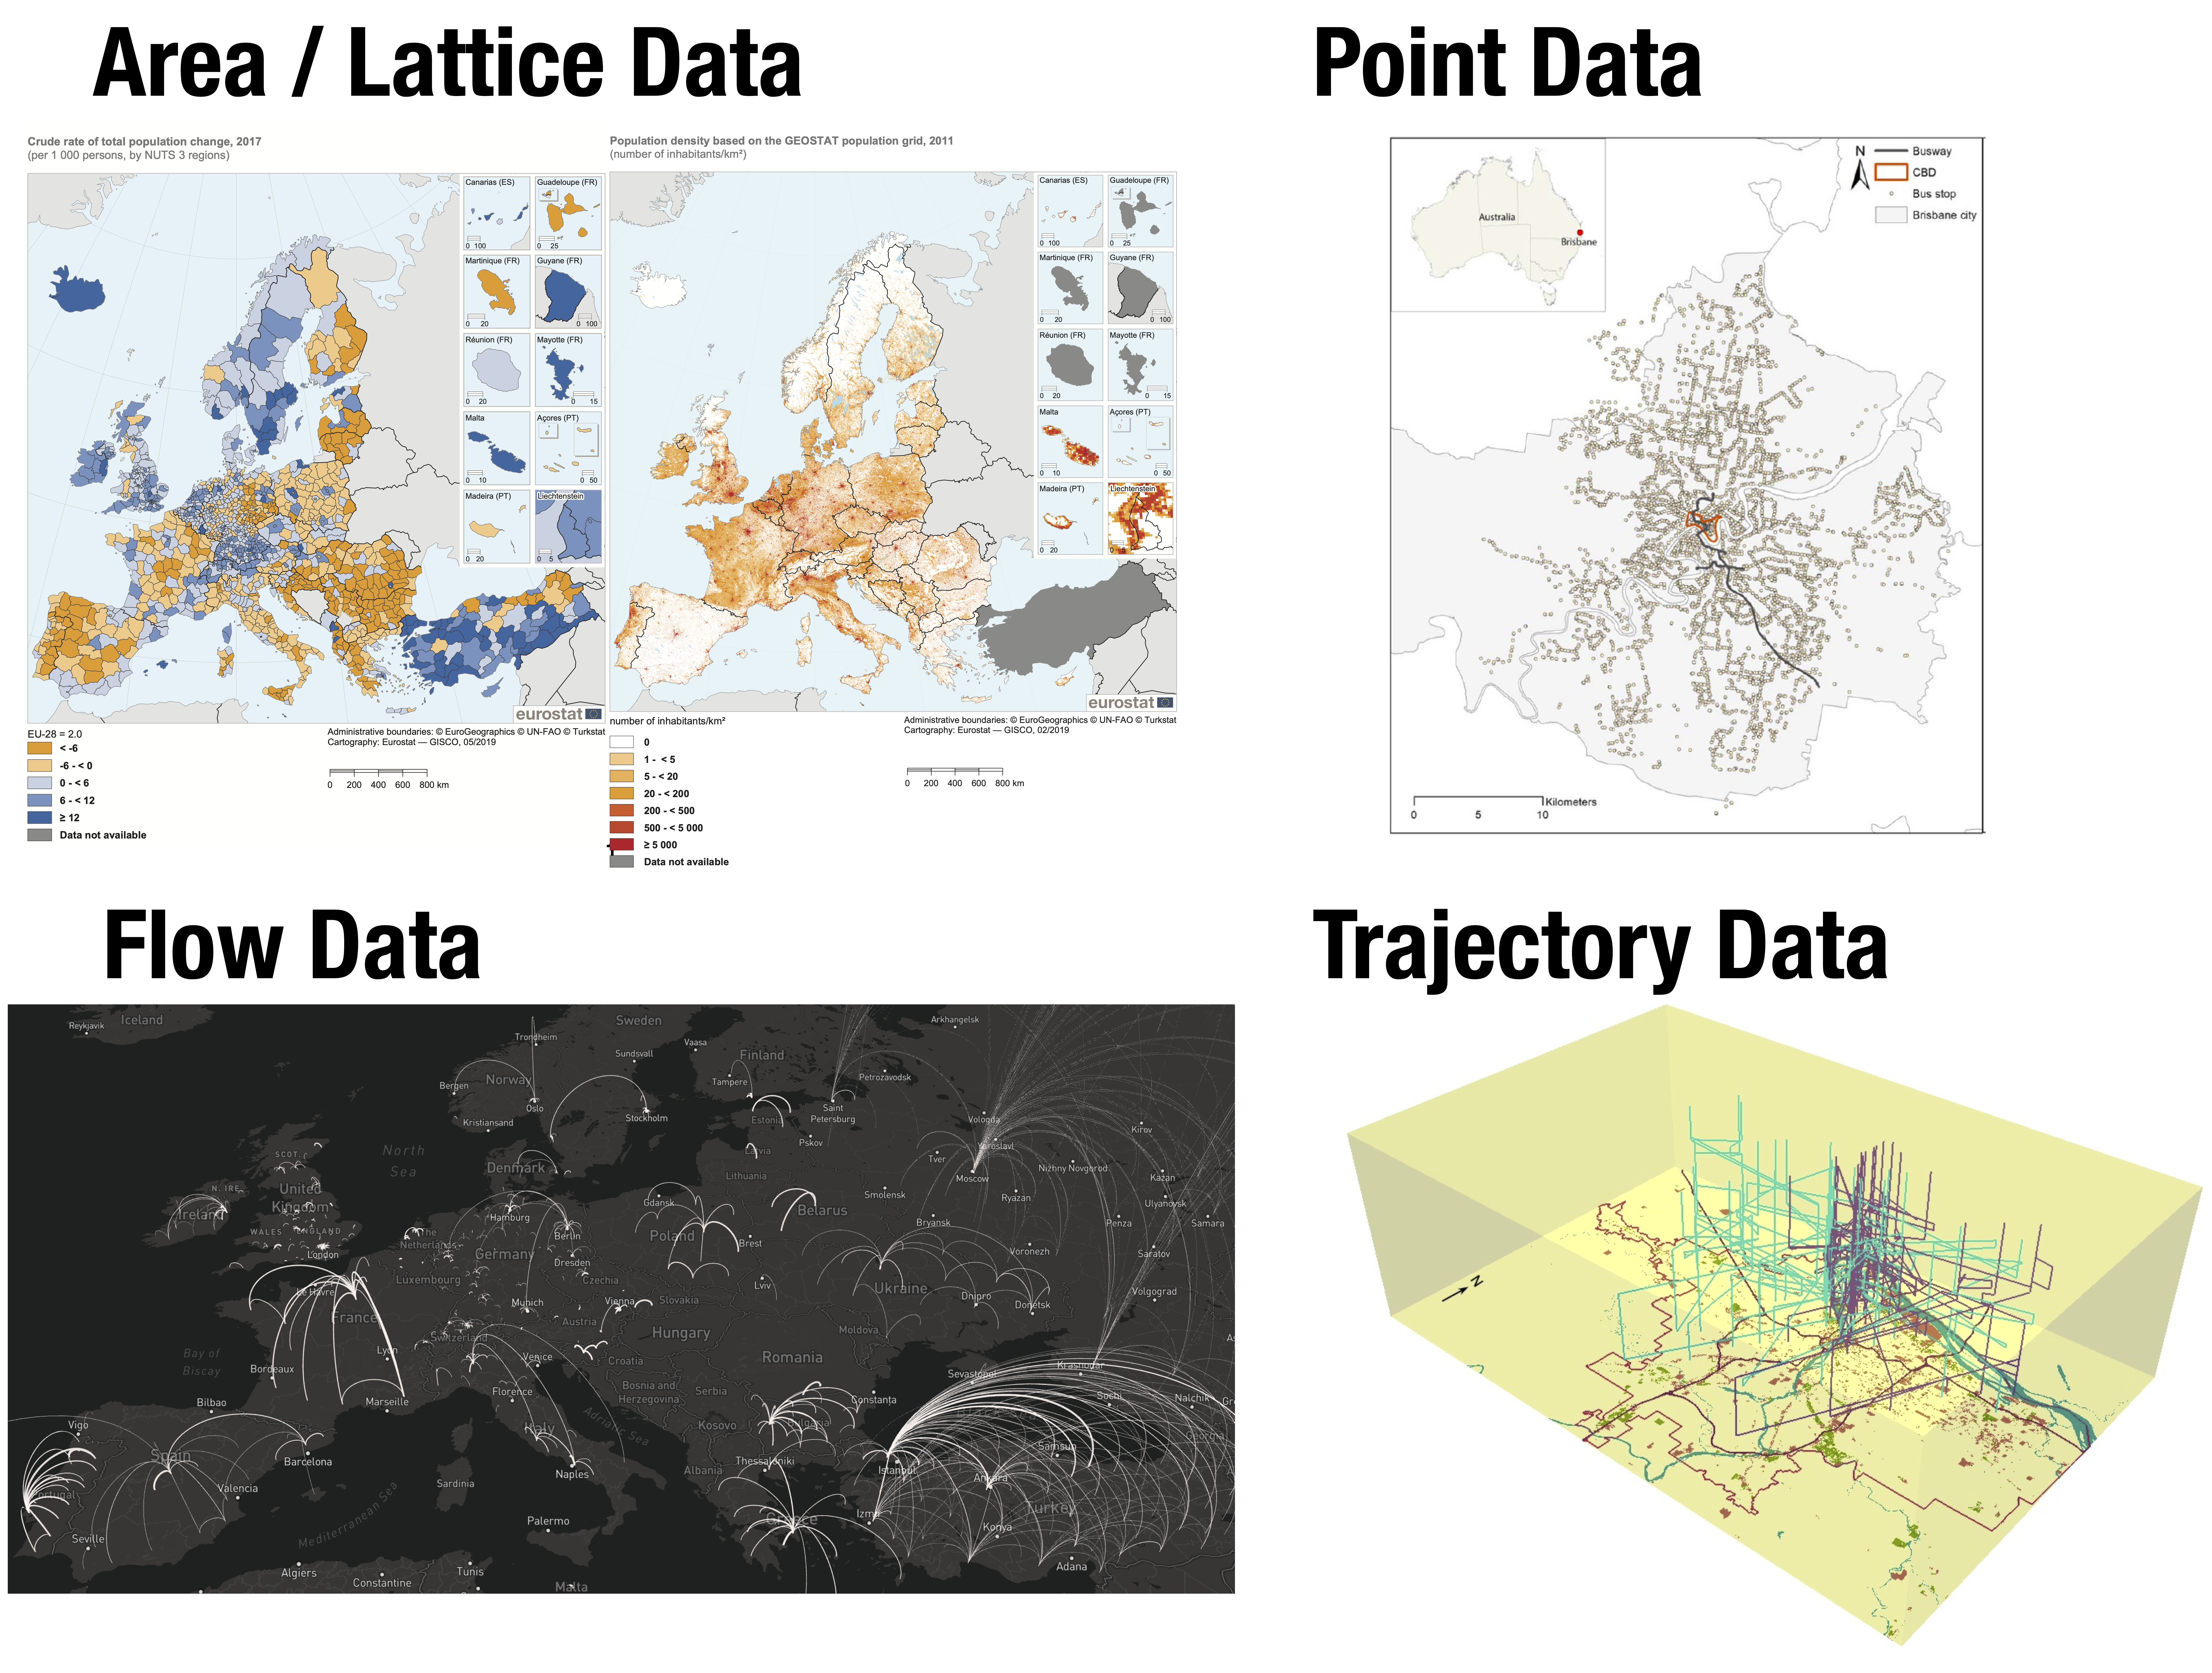
\includegraphics{./figs/ch1/datatypes.png}

}

\caption{Fig. 1. Data Types. Area / Lattice data source: Önnerfors et
al. (2019). Point data source: Tao et al. (2018). Flow data source: Rowe
and Patias (2020). Trajectory data source: Kwan and Lee (2004).}

\end{figure}

\emph{Lattice/Areal Data}. These data correspond to records of attribute
values (such as population counts) for a fixed geographical area. They
may comprise regular shapes (such as grids or pixels) or irregular
shapes (such as states, counties or travel-to-work areas). Raster data
are a common source of regular lattice/areal area, while censuses are
probably the most common form of irregular lattice/areal area. Point
data within an area can be aggregated to produce lattice/areal data.

\emph{Point Data}. These data refer to records of the geographic
location of an discrete event, or the number of occurrences of
geographical process at a given location. As displayed in Fig. 1,
examples include the geographic location of bus stops in a city, or the
number of boarding passengers at each bus stop.

\emph{Flow Data}. These data refer to records of measurements for a pair
of geographic point locations. or pair of areas. These data capture the
linkage or spatial interaction between two locations. Migration flows
between a place of origin and a place of destination is an example of
this type of data.

\emph{Trajectory Data}. These data record geographic locations of moving
objects at various points in time. A trajectory is composed of a single
string of data recording the geographic location of an object at various
points in time and each record in the string contains a time stamp.
These data are complex and can be classified into explicit trajectory
data and implicit trajectory data. The former refer to well-structured
data and record positions of objects continuously and intensively at
uniform time intervals, such as GPS data. The latter is less structured
and record data in relatively time point intervals, including
sensor-based, network-based and signal-based data (Kong et al. (2018)).

In this course, we cover analytical and modelling approaches for point,
lattice/areal and flow data. While we do not explicitly analyse
trajectory data, various of the analytical approaches described in this
book can be extended to incorporate time, and can be applied to model
these types of data. In Chapter @ref(sta), we describe approaches to
analyse and model spatio-temporal data. These same methods can be
applied to trajectory data.

\hypertarget{hierarchical-structure-of-data}{%
\section{Hierarchical Structure of
Data}\label{hierarchical-structure-of-data}}

The hierarchical organisation is a key feature of spatial data. Smaller
geographical units are organised within larger geographical units. You
can find the hierarchical representation of UK Statistical Geographies
on the
\href{https://geoportal.statistics.gov.uk/search?collection=Document\&sort=name\&tags=all(DOC_HRSG\%2CDEC_2020)}{Office
for National Statistics website}. In the bottom part of the output
below, we can observe a spatial data frame for Liverpool displaying the
hierarchical structure of census data (from the smallest to the
largest): Output Areas (OAs), Lower Super Output Areas (LSOAs), Middle
Super Output Areas (MSOAs) and Local Authority Districts (LADs). This
hierarchical structure entails that units in smaller geographies are
nested within units in larger geographies, and that smaller units can be
aggregated to produce large units.

\begin{verbatim}
Simple feature collection with 6 features and 4 fields
Geometry type: MULTIPOLYGON
Dimension:     XY
Bounding box:  xmin: 335071.6 ymin: 389876.7 xmax: 339426.9 ymax: 394479
Projected CRS: Transverse_Mercator
      OA_CD   LSOA_CD   MSOA_CD    LAD_CD                       geometry
1 E00176737 E01033761 E02006932 E08000012 MULTIPOLYGON (((335106.3 38...
2 E00033515 E01006614 E02001358 E08000012 MULTIPOLYGON (((335810.5 39...
3 E00033141 E01006546 E02001365 E08000012 MULTIPOLYGON (((336738 3931...
4 E00176757 E01006646 E02001369 E08000012 MULTIPOLYGON (((335914.5 39...
5 E00034050 E01006712 E02001375 E08000012 MULTIPOLYGON (((339325 3914...
6 E00034280 E01006761 E02001366 E08000012 MULTIPOLYGON (((338198.1 39...
\end{verbatim}

Next we quickly go through the components of the output above. The first
line indicates the type of feature and the number of rows (features) and
columns (fields) in the data frame, except for the geometry. The second
and third lines identify the type of geometry and dimension. The fourth
line \texttt{bbox} stands for bounding box and display the min and max
coordinates containing the Liverpool area in the data frame. The fifth
line \texttt{projected\ CRS} indicates the coordinate reference system
projection. If you would like to learn more about the various components
of spatial data frames, please see the \emph{R} \texttt{sf} package
vignette on
\href{https://r-spatial.github.io/sf/articles/sf1.html}{Simple
Features}.

\hypertarget{key-challenges}{%
\section{Key Challenges}\label{key-challenges}}

Major challenges exist when working with spatial data. Below we explore
some of the key longstanding problems data scientists often face when
working with geographical data.

\hypertarget{modifible-area-unit-problem-maup}{%
\subsection{Modifible Area Unit Problem
(MAUP)}\label{modifible-area-unit-problem-maup}}

The Modifible Area Unit Problem (MAUP) represents a challenge that has
troubled geographers for decades (Openshaw 1981). Two aspects of the
MAUP are normally recognised in empirical analysis relating to
\emph{scale} and \emph{zonation}. Fig. 2 illustrates these issues

\begin{itemize}
\item
  \emph{Scale} refers to the idea that a geographical area can be
  divided into geographies with differing numbers of spatial units.
\item
  \emph{Zonation} refers to the idea that a geographical area can be
  divided into the same number of units in a variety of ways.
\end{itemize}

\begin{figure}

{\centering \includegraphics{./figs/ch1/maup.png}

}

\caption{Fig. 2. MAUP effect. (a) scale effect; and, (b) zonation
effect. Source: loidl2016mapping.}

\end{figure}

The MAUP is a critical issue as it can impact our analysis and thus any
conclusions we can infer from our results (e.g. Fotheringham and Wong
1991). There is no agreed systematic approach on how to handle the
effects of the MAUP. Some have suggested to perform analyses based on
different existing geographical scales, and assess the consistency of
the results and identify potential sources of change. The issue with
such approach is that results from analysis at different scales are
likely to differ because distinct dimensions of a geographic process may
be captured at different scales. For example, in migration studies,
smaller geographies may be more suitable to capture residential mobility
over short distances, while large geographies may be more suitable to
capture long-distance migration. And it is well documented that these
types of moves are driven by different factors. While residential
mobility tends to be driven by housing related reasons, long-distance
migration is more closely related to employment-related motives
(Niedomysl 2011).

An alternative approach is to use the smallest geographical system
available and create random aggregations at various geographical scales,
to directly quantify the extent of scale and zonation. This approach has
shown promising results in applications to study internal migration
flows (Stillwell, Daras, and Bell 2018). Another approach involves the
production of ``meaningful'' or functional geographies that can more
appropriately capture the process of interest. There is an active area
of work defining functional labour markets (Casado-Dı́az,
Martı́nez-Bernabéu, and Rowe 2017), urban areas (Arribas-Bel,
Garcia-López, and Viladecans-Marsal 2019) and various forms of
geodemographic classifications (Singleton and Spielman 2014; Patias,
Rowe, and Cavazzi 2019). However there is the recognition that none of
the existing approaches resolve the effects of the MAUP and recently it
has been suggested that the most plausible `solution' would be to ignore
the MAUP (Wolf et al. 2020).

\hypertarget{ecological-fallacy}{%
\subsection{Ecological Fallacy}\label{ecological-fallacy}}

Ecological fallacy is an error in the interpretation of statistical data
based on aggregate information. Specifically it refers to inferences
made about the nature of specific individuals based solely on statistics
aggregated for a given group. It is about thinking that relationships
observed for groups necessarily hold for individuals. A key example is
Robinson (1950) who illustrates this problem exploring the difference
between ecological correlations and individual correlations. He looked
at the relationship between country of birth and literacy. Robinson
(1950) used the percent of foreign-born population and percent of
literate population for the 48 states in the United States in 1930. The
ecological correlation based on these data was \texttt{0.53}. This
suggests a positive association between foreign birth and literacy, and
could be interpreted as foreign born individuals being more likely to be
literate than native-born individuals. Yet, the correlation based on
individual data was negative \texttt{-0.11} which indicates the
opposite. The main point emerging from this example is to carefully
interpret analysis based on spatial data and avoid making inferences
about individuals from these data.

\hypertarget{spatial-dependence}{%
\subsection{Spatial Dependence}\label{spatial-dependence}}

Spatial dependence refers to the spatial relationship of a variable's
values for a pair of locations at a certain distance apart, so that
these values are more similar (or less similar) than expected for
randomly associated pairs of observations (Anselin 1988). For example,
we could think of observed patterns of ethnic segregation in an area are
a result of spillover effects of pre-existing patterns of ethnic
segregation in neighbouring areas. Chapter @ref(spatialecon) will
illustrate approach to explicitly incorporate spatial dependence in
regression analysis.

\hypertarget{spatial-heterogeneity}{%
\subsection{Spatial Heterogeneity}\label{spatial-heterogeneity}}

Spatial heterogeneity refers to the uneven distribution of a variable's
values across space. Concentration of deprivation or unemployment across
an area are good examples of spatial heterogeneity. We illustrate
various ways to visualise, explore and measure the spatial distribution
of data in multiple chapters. We also discuss on potential modelling
approaches to capture spatial heterogeneity in Chapters
@ref(spatialecon), @ref(mlm1) and @ref(sta).

\hypertarget{spatial-nonstationarity}{%
\subsection{Spatial nonstationarity}\label{spatial-nonstationarity}}

Spatial nonstationarity refers to variations in the relationship between
an outcome variable and a set of predictor variables across space. In a
modelling context, it relates to a situation in which a simple
``global'' model is inappropriate to explain the relationships between a
set of variables. The geographical nature of the model must be modified
to reflect local structural relationships within the data. For example,
ethnic segregation has been positively associated with employment
outcomes in some countries pointing to networks in pre-existing
communities facilitating access to the local labour market. Inversely
ethnic segregation has been negatively associated with employment
outcomes pointing to lack of integration into the broader local
community. We illustrate various modelling approaches to capture spatial
nonstationarity in Chapters @ref(mlm2) and @ref(gwr).

\bookmarksetup{startatroot}

\hypertarget{summary}{%
\chapter{Summary}\label{summary}}

In summary, this book has no content whatsoever.

\begin{Shaded}
\begin{Highlighting}[]
\DecValTok{1} \SpecialCharTok{+} \DecValTok{1}
\end{Highlighting}
\end{Shaded}

\begin{verbatim}
[1] 2
\end{verbatim}

\bookmarksetup{startatroot}

\hypertarget{references}{%
\chapter*{References}\label{references}}
\addcontentsline{toc}{chapter}{References}

\hypertarget{refs}{}
\begin{CSLReferences}{1}{0}
\leavevmode\vadjust pre{\hypertarget{ref-anselin1988spatial}{}}%
Anselin, Luc. 1988. \emph{Spatial Econometrics: Methods and Models}.
Vol. 4. Springer Science \& Business Media.

\leavevmode\vadjust pre{\hypertarget{ref-arribas2019building}{}}%
Arribas-Bel, Daniel, M-À Garcia-López, and Elisabet Viladecans-Marsal.
2019. {``Building (s and) Cities: Delineating Urban Areas with a Machine
Learning Algorithm.''} \emph{Journal of Urban Economics}, 103217.

\leavevmode\vadjust pre{\hypertarget{ref-casado2017evolutionary}{}}%
Casado-Dı́az, José Manuel, Lucas Martı́nez-Bernabéu, and Francisco Rowe.
2017. {``An Evolutionary Approach to the Delimitation of Labour Market
Areas: An Empirical Application for Chile.''} \emph{Spatial Economic
Analysis} 12 (4): 379--403.

\leavevmode\vadjust pre{\hypertarget{ref-fotheringham1991modifiable}{}}%
Fotheringham, A Stewart, and David WS Wong. 1991. {``The Modifiable
Areal Unit Problem in Multivariate Statistical Analysis.''}
\emph{Environment and Planning A} 23 (7): 1025--44.

\leavevmode\vadjust pre{\hypertarget{ref-kong2018big}{}}%
Kong, Xiangjie, Menglin Li, Kai Ma, Kaiqi Tian, Mengyuan Wang, Zhaolong
Ning, and Feng Xia. 2018. {``Big Trajectory Data: A Survey of
Applications and Services.''} \emph{IEEE Access} 6: 58295--306.

\leavevmode\vadjust pre{\hypertarget{ref-kwan2004geovisualization}{}}%
Kwan, Mei-Po, and Jiyeong Lee. 2004. {``Geovisualization of Human
Activity Patterns Using 3d GIS: A Time-Geographic Approach.''}
\emph{Spatially Integrated Social Science} 27: 721--44.

\leavevmode\vadjust pre{\hypertarget{ref-niedomysl2011migration}{}}%
Niedomysl, Thomas. 2011. {``How Migration Motives Change over Migration
Distance: Evidence on Variation Across Socio-Economic and Demographic
Groups.''} \emph{Regional Studies} 45 (6): 843--55.

\leavevmode\vadjust pre{\hypertarget{ref-onnerfors2019eurostat}{}}%
Önnerfors, Åsa, Mariana Kotzeva, Teodóra Brandmüller, et al. 2019.
{``Eurostat Regional Yearbook 2019 Edition.''}

\leavevmode\vadjust pre{\hypertarget{ref-openshaw1981modifiable}{}}%
Openshaw, Stan. 1981. {``The Modifiable Areal Unit Problem.''}
\emph{Quantitative Geography: A British View}, 60--69.

\leavevmode\vadjust pre{\hypertarget{ref-patias2019scalable}{}}%
Patias, Nikos, Francisco Rowe, and Stefano Cavazzi. 2019. {``A Scalable
Analytical Framework for Spatio-Temporal Analysis of Neighborhood
Change: A Sequence Analysis Approach.''} In \emph{International
Conference on Geographic Information Science}, 223--41. Springer.

\leavevmode\vadjust pre{\hypertarget{ref-robinson1950ecological}{}}%
Robinson, WS. 1950. {``Ecological Correlations and Individual
Behavior.''} \emph{American Sociological Review} 15 (195): 351--57.

\leavevmode\vadjust pre{\hypertarget{ref-rowe2020mapping}{}}%
Rowe, Francisco, and Nikos Patias. 2020. {``Mapping the Spatial Patterns
of Internal Migration in Europe.''} \emph{Regional Studies, Regional
Science} 7 (1): 390--93.

\leavevmode\vadjust pre{\hypertarget{ref-singleton2014past}{}}%
Singleton, Alexander D, and Seth E Spielman. 2014. {``The Past, Present,
and Future of Geodemographic Research in the United States and United
Kingdom.''} \emph{The Professional Geographer} 66 (4): 558--67.

\leavevmode\vadjust pre{\hypertarget{ref-stillwell2018spatial}{}}%
Stillwell, John, Konstantinos Daras, and Martin Bell. 2018. {``Spatial
Aggregation Methods for Investigating the MAUP Effects in Migration
Analysis.''} \emph{Applied Spatial Analysis and Policy} 11 (4):
693--711.

\leavevmode\vadjust pre{\hypertarget{ref-tao2018travel}{}}%
Tao, Sui, Jonathan Corcoran, Francisco Rowe, and Mark Hickman. 2018.
{``To Travel or Not to Travel:`weather'is the Question. Modelling the
Effect of Local Weather Conditions on Bus Ridership.''}
\emph{Transportation Research Part C: Emerging Technologies} 86:
147--67.

\leavevmode\vadjust pre{\hypertarget{ref-wolf2020quantitative}{}}%
Wolf, Levi John, Sean Fox, Rich Harris, Ron Johnston, Kelvyn Jones,
David Manley, Emmanouil Tranos, and Wenfei Winnie Wang. 2020.
{``Quantitative Geography III: Future Challenges and Challenging
Futures.''} \emph{Progress in Human Geography}, 0309132520924722.

\leavevmode\vadjust pre{\hypertarget{ref-xie2018r}{}}%
Xie, Yihui, Joseph J Allaire, and Garrett Grolemund. 2018. \emph{R
Markdown: The Definitive Guide}. CRC Press.

\end{CSLReferences}



\end{document}
